\begin{surferPage}[Double Cone]{A Double Cone}
   %As explained in the introduction to this gallery a surface is called
	Kako je obja\v{s}njeno u uvodu u ovu galeriju, ka\v{z}emo da je ploha
    %\emph{non--singular} or smooth if it does not have any apexes
		\emph{nesingularna} ili glatka ako nema vrhove
    %(such points are called singularities).
		(takve to\v{c}ke zovemo singularitetima).
    %For example, a sphere or a torus (two leftmost pictures below):
		Takve plohe su sfera i torus (dvije lijeve slike ispod):
    \begin{center}
      \begin{tabular}{@{}c@{}c@{}c@{}c@{}}
        \begin{tabular}{@{}c}
          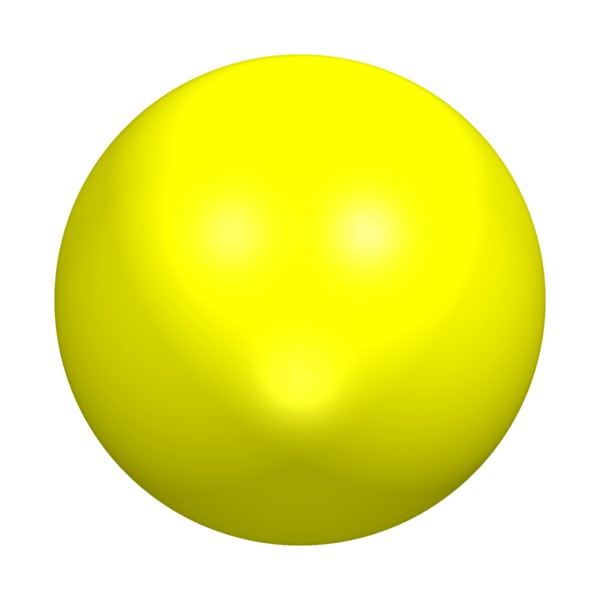
\includegraphics[width=1.4cm]{./../../common/images/kugel}
        \end{tabular}
        &
        \begin{tabular}{@{}c}
          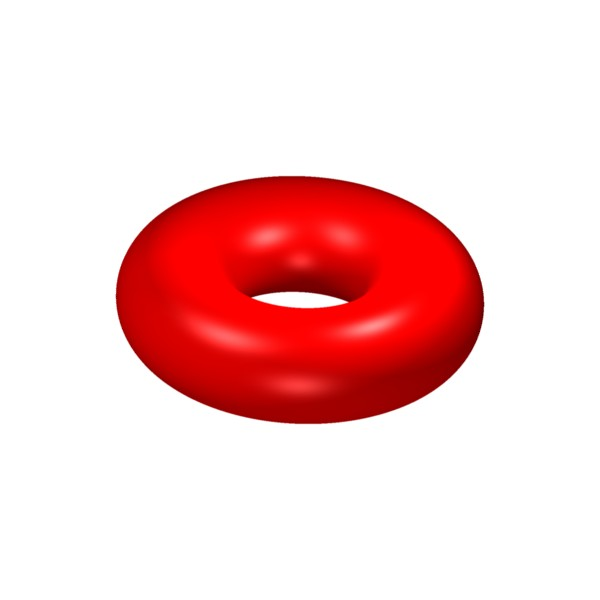
\includegraphics[width=1.4cm]{./../../common/images/torus}
        \end{tabular}
        &
        \begin{tabular}{c@{}}
          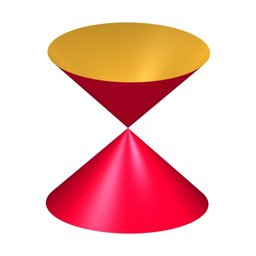
\includegraphics[width=1.4cm]{./../../common/images/kegel}
        \end{tabular}
      \end{tabular}
    \end{center}
     %The double cone (rightmost picture) is the simplest singularity; it is the only singularity which can be described by an equation of
		Dvostruki konus (desna slika) je najjednostavniji singularitet; to je jedini singularitet koji se mo\v{z}e opisati
		%degree $2$:
		jednad\v{z}bom stupnja $2$:
    \[x^2+y^2-z^2=0.\]
    %When changing this equation slightly by replacing the $0$ with a small value
		Zamijenimo li u ovoj jednad\v{z}bi $0$ nekom malom vrijedno\v{s}\'{c}u $a\neq 0$,
		%the double cone transforms into one of the two types of
		dvostruki konus postaje jedan od dva tipa hiperboloida,
    %hyperboloids, depending on the sign of $a$:
		u ovisnosti o predznaku od $a$:
    \begin{center}
      \begin{tabular}{@{}c@{\ }c@{\ }c@{\ }c@{\ }c@{}}
        \begin{tabular}{@{}c@{}}
          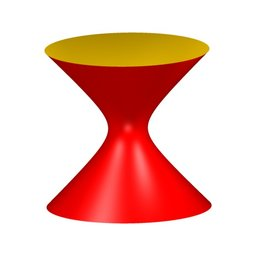
\includegraphics[width=1.2cm]{./../../common/images/A1pm_2}
        \end{tabular}
        &
        $\leftarrow$
        &
        \begin{tabular}{@{}c@{}}
          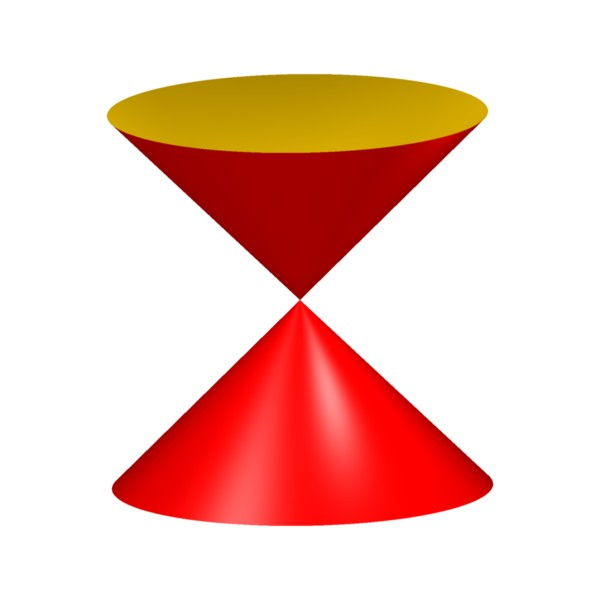
\includegraphics[width=1.2cm]{./../../common/images/A1pm_1} 
        \end{tabular}
        &
        $\rightarrow$
        &
        \begin{tabular}{@{}c@{}}
          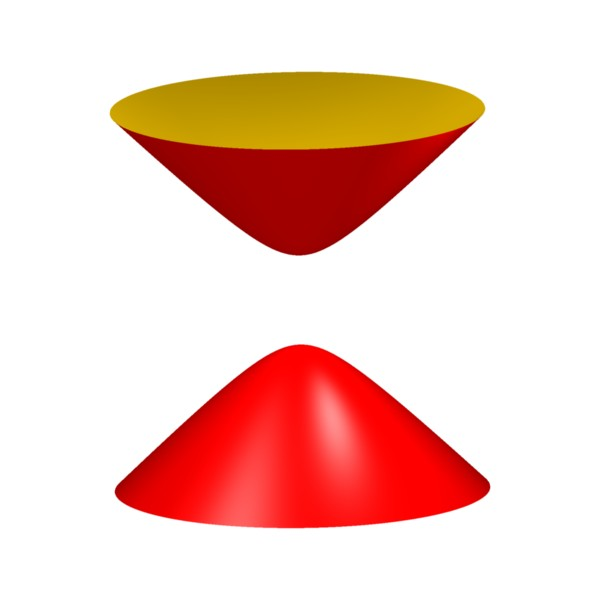
\includegraphics[width=1.2cm]{./../../common/images/A1pm_0}
        \end{tabular}
      \end{tabular}
    \end{center}
   %A surface of degree $2$ cannot have more than one singularity, i.e.\ $\mu(2)=1$.
	Ploha stupnja $2$ ne mo\v{z}e imati vi\v{s}e od jednog singulariteta, tj. $\mu(2)=1$.
\end{surferPage}
